\documentclass[acmtog, authorversion]{acmart}

\usepackage{booktabs} % For formal tables
\usepackage{hyperref}
\usepackage{placeins}

% TOG prefers author-name bib system with square brackets
\citestyle{acmauthoryear}
\setcitestyle{square}

\usepackage[ruled]{algorithm2e} % For algorithms
\renewcommand{\algorithmcfname}{ALGORITHM}
\SetAlFnt{\small}
\SetAlCapFnt{\small}
\SetAlCapNameFnt{\small}
\SetAlCapHSkip{0pt}
\IncMargin{-\parindent}

% Metadata Information
\acmYear{2017}
\acmMonth{9}

% Copyright
%\setcopyright{acmcopyright}
%\setcopyright{acmlicensed}
\setcopyright{rightsretained}
%\setcopyright{usgov}
%\setcopyright{cagov}
%\setcopyright{cagovmixed}

% Document starts
\begin{document}
% Title portion
\title{Finding trends in open-source software by visualizing collaboration over time}

\author{Rick Proost}
\affiliation{%
\institution{Delft University of Technology}
\country{The Netherlands}}
\email{rpjproost@gmail.com}

\author{Vincent Robbemond}
\affiliation{%
\institution{Delft University of Technology}
\country{The Netherlands}}
\email{vincentrobbemond@gmail.com}

\author{Wim Spaargaren}
\affiliation{%
\institution{Delft University of Technology}
\country{The Netherlands}}
\email{wim_spaargaren@live.nl}

\begin{abstract}
The open-source software community has seen a lot of growth in the past years and remains to grow.
Collaboration platforms like GitHub provide easy access to all open-source project data by providing an API, making open-source development data for over 24 million users accessible.
While this data has been available for some time, there has not been done a lot of research into how this data can be applied to bring insights in the way developers collaborate.
Developer collaboration has become a bigger point of discussion since the rise of Globally Distributed Software Engineering and can benefit from insights derived from this readily available data.
This paper describes the building of an online platform to provide visualizations of collaboration on the open source software platform GitHub.
In addition, this work explores the evolution of developer activity for open source software project.
This exploratory research answers questions about the evolution of developer activity in the developer community and the way geographic distance between repository owner and developer influences the amount of commits made by a developer.
\end{abstract}

\keywords{Data Visualization, GitHub, Open Source Software, Collaboration}

\maketitle

\section{Introduction}
In the past few years the open-source software(OSS) community and development activity in OSS have grown.
According to GitHub \cite{GHOctoverse}, in 2016, there were over 5.8 million users engaged in activities relating to public repositories.
GitHub defines these activities as "some activity within the last year, for example, code committed, a comment created, a repository starred, or an issue opened" \cite{GHOctoverse}.

With GitHub providing programmatic access to all OSS repository and user data\cite{GHAPI}, it is possible to collect and manipulate this data to get more insights into the way the OSS community collaborates on GitHub.
These new insights can be applied to improve or develop new software development methods. It is also possible to improve existing collaboration platforms like GitHub or coding standards, which improve developer collaboration \cite{Jermakovics2013}.
Outside of the OSS community, a better understanding of how the OSS community functions helps commercial IT projects adopt typical OSS practices, for example, promoting open collaboration \cite{Kalliamvakou:2015:OSC:2818754.2818825}, and may help IT planners make more informed decisions and develop more effective strategies for using OSS software \cite{madey2002}.

One way for researchers to analyze the gathered data, is by visualizing it \cite{Heller}.
One of the objective of the Software Visualization field is to aid stakeholders in developing a greater understanding of software systems, their evolution and development.
"The basic idea of visual data exploration is to present the data in some visual form, allowing the human to get insight into the data, draw conclusions, and directly interact with the data.
Visual data mining techniques have proven to be of high value in exploratory data analysis and they also have high potential for exploring large databases." \cite{981847}.
To give developers insights in repositories, GitHub also provides some visualizations. 
One of these visualization is "Developer Contribution", which shows amount of commits made during a period of time.
Up until september 2017 there have not been a lot of tools or platforms which provide visual insight into collaboration over time on a specific repository for example.
Tools which are available are outdated \cite{Heller} or not sufficient. For example a visualization of GitHub's newest and most popular repositories \cite{donnemartin2016}, a GitHub repository history visualizer \cite{artzub2013}, and a repository stats visualizer \cite{bajaj2013}.
Although these examples are visualization tools for GitHub, they provide insufficient information on developer collaboration in OSS projects.

Popular statistics that for example Github \cite{GHOctoverse} and StackOverflow \cite{StackOverflow2017} share are mostly quantitative studies on amount of people using the platform and for what reason.
These statistics do not offer insight into developer collaboration and trends on a more detailed level, although the data found on these platforms can reveal these latent factors.

Therefore, the main contribution of this paper is to provide a tool which stakeholders can leverage to gain insights into OSS projects and developer collaboration.
In particular, available data will show where developers are located, this will help identifying possible cultural differences between collaborators which is important to prevent coordination and collaboration problems \cite{Mishra2014}.

\textbf{This paper focuses on finding different patterns in OSS development by visualizing collaboration over time}

Since this is a broad subject, this paper focuses on answering two, more specific questions, with the help of the aforementioned tool.
Answers to the related questions will not provide a conclusive answer to the main question asked but in turn invite others to extend and explore this subject.

GitHub statistics show that 24 million people are making use of GitHub. 
These users are divided over 200 countries in all continents, with Asia (7.1 million), North-America (5.9 million) and Europe (5.3 million) hosting the largest amount of users \cite{GHOctoverse}.
StackOverflow developer survey 2017 \cite{StackOverflow2017} has similar results, showing big clusters in the USA, Western-Europa and India.
Countries with the highest numbers of users registered in 2017 on GitHub are the USA (1.2 million) and China (0.7 million) \cite{GHOctoverse}.
Different countries have different growth rates of GitHub users which registered in 2017. 
Identifying and looking into countries with the highest growth rates could lead to interesting insights.
Such insight could be identifying countries with a high growth in software developers, which would be interesting for IT companies, because there has been a developer shortage for years and companies are competing for the best and the brightest.
By adding a temporal element to active number of developers per country, it will be possible to tell in which countries the number of active developers in open-source software evolves faster.
Analyzing the trend in developer growth can be leveraged by OSS stakeholders. For example, companies seeking open-source developers to outsource software development to \cite{haefliger2008code}.

Underlying reasons can then be researched for this rise in popularity.

Therefore we first explore the question: \textbf{Does the number of active developers in the OSS community evolve faster for different countries?}

Distributed software engineering is an upcoming way of developing software.
One of the problems with distributed software engineering however is that developers are located on different development locations. 
Because of this, the second area we explore is developer collaboration, by analyzing collaboration links.
Collaboration links are defined as links between developers who add contributions consecutively to the same project.
By adding a temporal component to visualizing collaboration links, it becomes possible to see the way developer collaboration changes over time.
At the same time it becomes possible to see if the distance between developers working on the same project has influence on collaboration, and further exploring the impact of cultural differences in software development \cite{Mishra2014}.

The second question we explore is: \textbf{Does the number of commits made by a developer evolve faster for different countries?}

The answers could be derived from visualizing the data in such a way researchers can make well substantiated and testable hypotheses.
Therefore, the main outcome of this work is an online platform that allows users to visualizes evolution on collaboration of open source development on Github over time.

\section{Related work}
Analysis of developer collaboration is already done in some variations, but it presents some challenges while collaboration relationships are initially not known. 
In this paper collaborations are discovered by identifying developers with the same interest by grouping developers that star the same repository on github, or do consecutive commits.
This technique is also used by \cite{Heller}, which began research in visualizing developer collaboration. 
There are also other techniques like identifying developers that work on the same file by investigating Version Control Systems (VCS) \cite{Jermakovics2013}.
Most researches done do not add detailed visualizations, however, less scientific researches like \cite{GHOctoverse} and \cite{StackOverflow2017} give visualized statistics on their own platform.
Again other researches focus more on the social aspect of developer collaboration like a later work of Jermakovics \cite{Jermakovics2011}.
This work demonstrates an approach of how to construct a network and applies filtering techniques.
None of this scientific work offer an actual platform however where these collaborations and trends can be visualized dynamically however. By providing this platform, researchers are enabled to find more latent factors in the data gathered from the  top 1000 repositories.

\section{Methodology}
To answer the research questions,  a set of large repositories (i.e. repositories with the most GitHub stars and/or collaborators) on the open source software platform GitHub have been chosen.
A data scraper was built to retrieve data from the previously mentioned repositories.
The scraped data includes (but is not limited to) the owner, contributors and collaborators of the repository.
Aside from user information, commits are gathered for the repositories to compare statistics in different time frames, like how many commits are done from month to month or where consecutive commits are originated from.

A web-based service customly created is used to efficiently search and navigate repositories or GitHub users.
The retrieved data is displayed in multiple forms like geolocations for collaborators on  interactive maps among which Google Maps \cite{GoogleMaps}, D3 \cite{D3} and activity for a project in a graph with a temporal component.
Different ways of linking users and repositories are experimented with and results are published and available online at \cite{githubvisualizerovertime}.

By creating this web-based service, new insights emerge for collaboration in open source software development.
This reveals trends in software collaboration, activity and collaboration links over time.
In addition, this provides new ways for researchers to retrieve insights in open source software development collaboration statistics and form new hypotheses by analyzing the dynamic visualizations.

\section{Implementation}
The first step in answering the research questions, is the retrieval of data from the software development platform GitHub.
This data is gathered by using the GitHub REST API\cite{GHAPI}.
According to Octoverse \cite{GHOctoverse} in 2016 there were nearly 20 million software repositories. 
To decide the usage of repositories, the most starred repositories are chosen. Stars give an indication to the popularity of a repository and therefore have higher chances on relatively more activity than less popular repositories.
The storage of this amount of data goes beyond the scope of this research paper.
The repositories retrieved are therefore limited to the top 1000 starred repositories on GitHub.
The top 1000 starred repositories were listed and specified at \cite{gitstar} on september 2017.
Retrieval of data for these projects is done by a custom data scraper, the database dump can be found at  \cite{githubvisualizerovertime}.
The scraper first retrieves the repository data using the projects resource\cite{GHAPI}, afterwards all the commits with the corresponding user and at last the location are translated into geocoordinates.
The GitHub platform allows a user to specify a location on their profile, where user location is stored as plain text.
This means not all users have a location and some locations may not be as specific as others.
Commit data contains a message which is mostly used to describe the change and a timestamp denoting commit time.
Commit author and committer data is also available, therefore it is possible to make a distinction if necessary.
Finally, another custom scraper retrieved all star events for each repository using the repository stargazer resource\cite{GHAPI}.
A stargazer is a user who stars a certain repository, so Developer A stars Repository B, therefore A is now in the list of stargazers of B.
The star events depicts another way of activity in open source software development and can be of value when visualizing activity data. The developers starring the same repository in the same timespan also share a relationship which can be visualized.

The self developed data scraper can be found at \cite{githubvisualizerovertime} together with a database dump for the top 1000 starred repositories of September 2017.
This Golang scripts provide functionality to gather both commits and stars for projects.
Projects which data needs to be retrieved for, can be specified in two ways, by providing a json file with project names, or by reading repository names from a self provided database.
For each project, commits and stars from the current date until the last stored commit in the database are retrieved and stored in the specified database.
Detailed build instructions are provided in the README file.
\begin{figure*}
\center
\frame{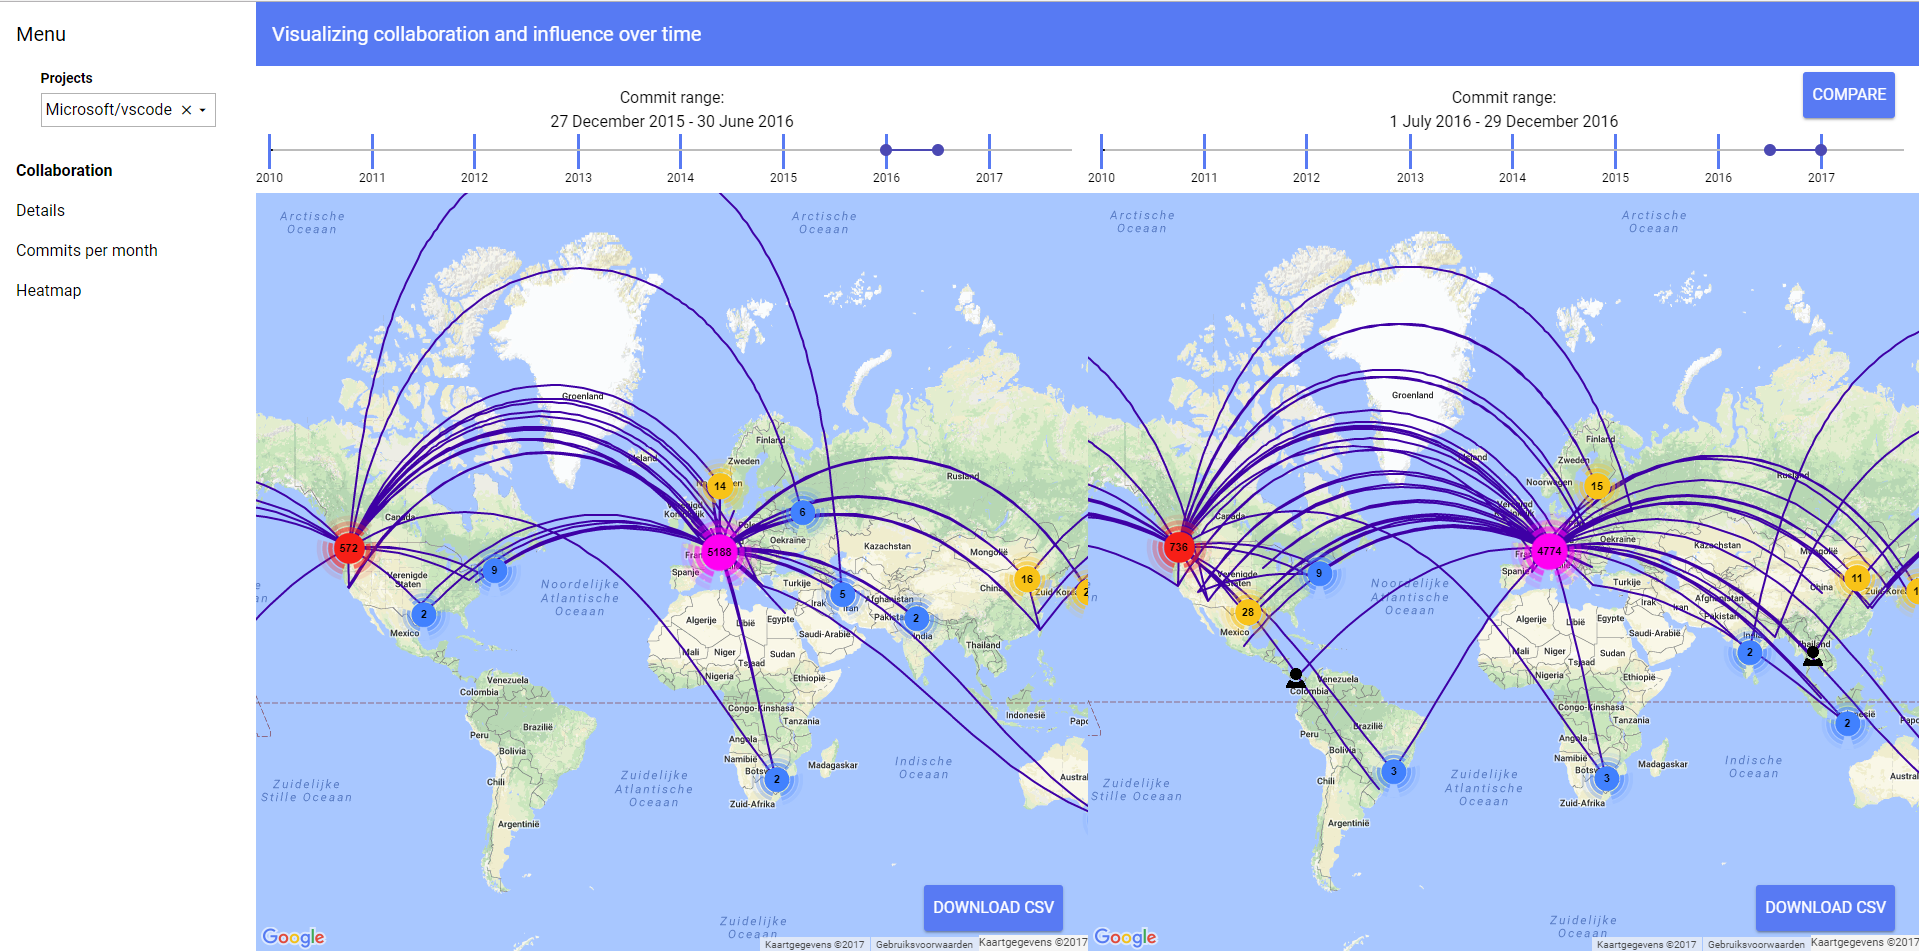
\includegraphics[scale=0.35]{images/vscode-compare.PNG}}
\caption{Example visualization of developer collaboration comparison for VSCode}
\label{fig:collaboration}
\end{figure*}

Figure ~\ref{fig:collaboration} shows a visualization example for the repository Visual Studio Code.
Markers depict commits, with a location of where the author of the commit is located.
Lines depict collaboration between developers.
This collaboration is defined as successive commits done by collaborators working on the same project.
When at a lower zoom level, nodes get un-grouped and lines between individual developers will be shown.
In the top of the page a timeline is shown.
In the timeline a timespan can be selected.
After selecting a timespan, commits within this timespan are shown on the map.
A download CSV button is added to download the shown commit data as CSV file.
This way users of the platform can further analyze the data shown.
By pressing the compare button, two visualizations can be shown next to each other.
In figure  ~\ref{fig:collaboration} commits from the first half of 2016 are compared to commits of the second half of 2016.
\begin{figure*}
\center
\frame{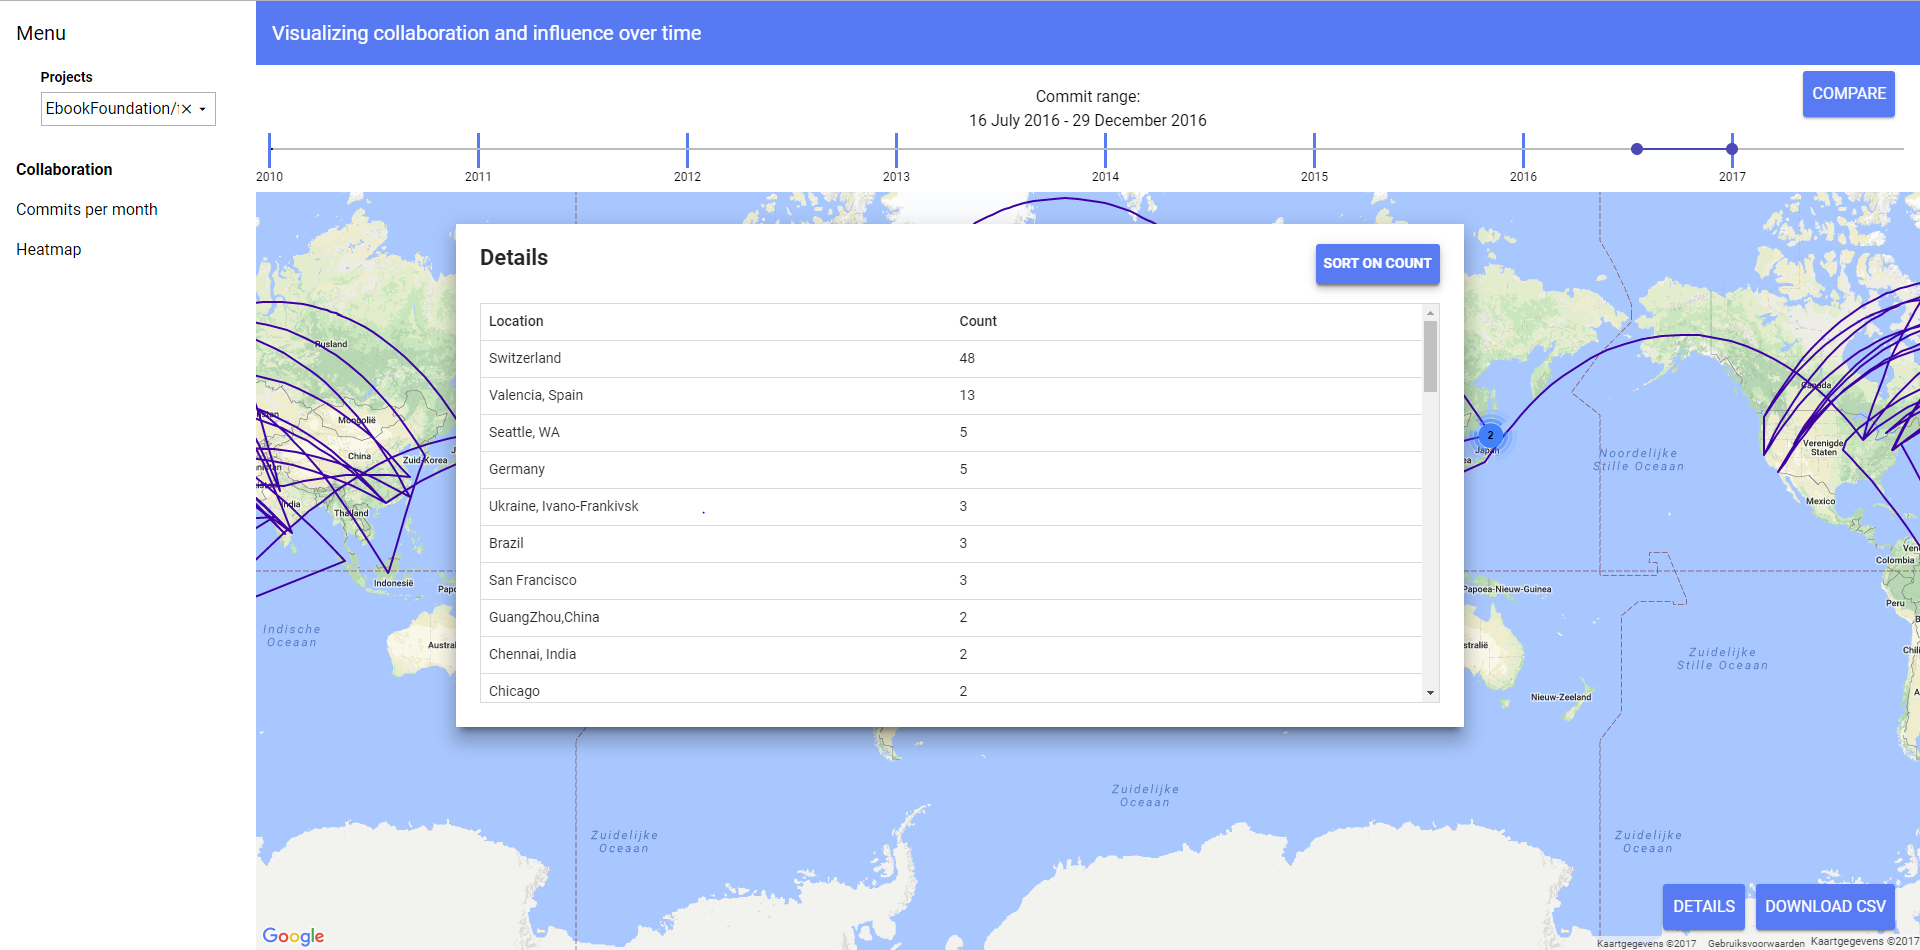
\includegraphics[scale=0.35]{images/details-popup-ebook-foundation.PNG}}
\caption{Example details popup}
\label{fig:details}
\end{figure*}

A second button is provided to show details about the commits currently shown on the map.
By pressing the details button, a dialog is created with information about the number of commits per location, as shown in ~\ref{fig:details}.
In this example commits of the second half of 2016 are shown.
In the dialog a sort on count button is added to sort the commit details in ascending or descending order.

\begin{figure*}
\center
\frame{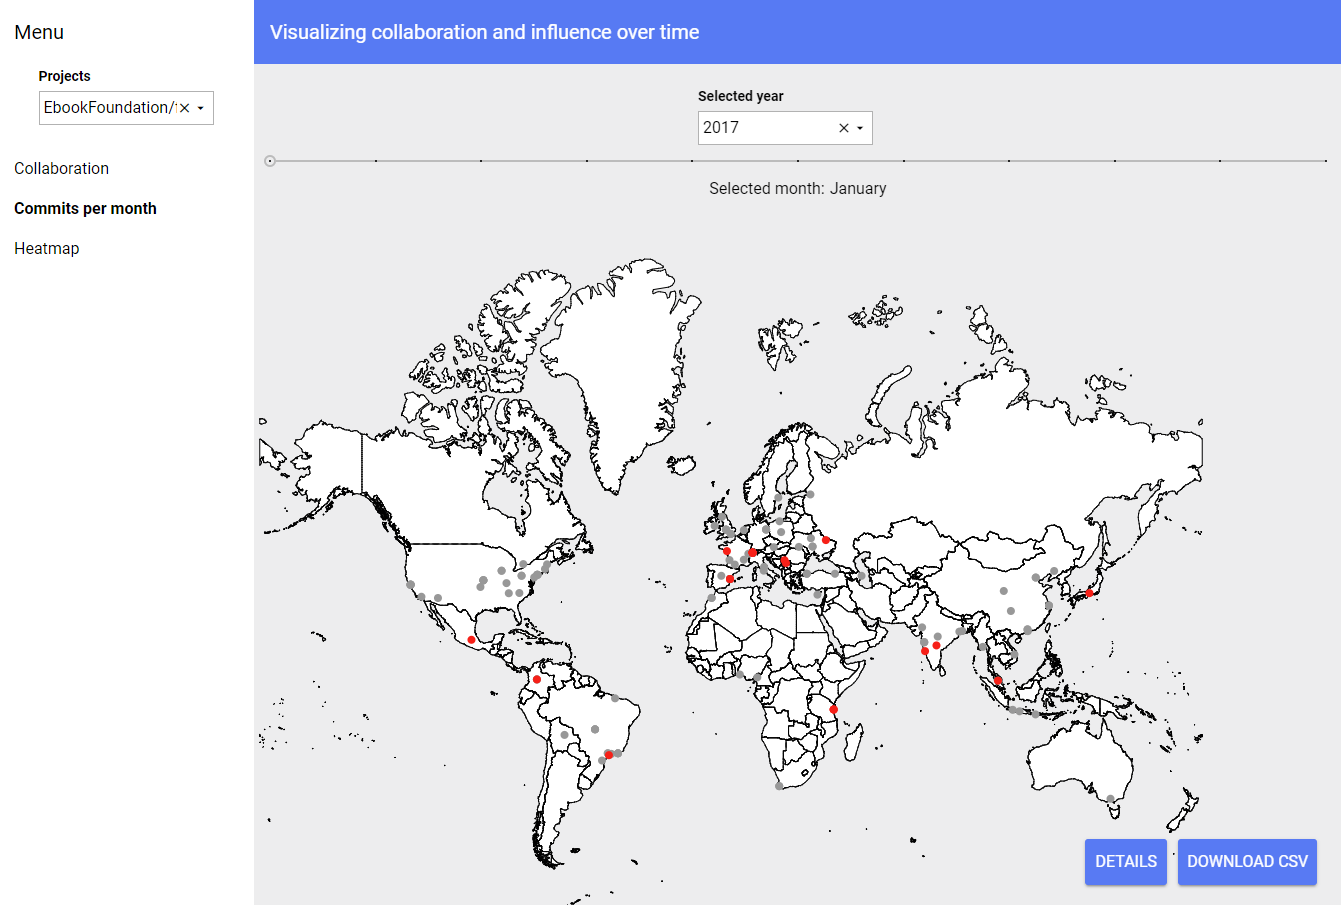
\includegraphics[scale=0.4]{images/d3-example-rails.PNG}}
\caption{Example visualization of commits per month}
\label{fig:commits-period}
\end{figure*}

Figure ~\ref{fig:commits-period} shows an example of a map built with the D3 library.
Every dot represents a commit belonging to a repository in a year span, which can be selected by selecting a year in the dropdown menu.
Red dots represent commits made during the month selected in the second slider.
Beneath this slider the selected month is stated.
By adjusting the month slider, it is possible to visualize how commits change per month for a project.
As well as the first visualization both the details button and the download csv button are provided.

\begin{figure*}
\center
\frame{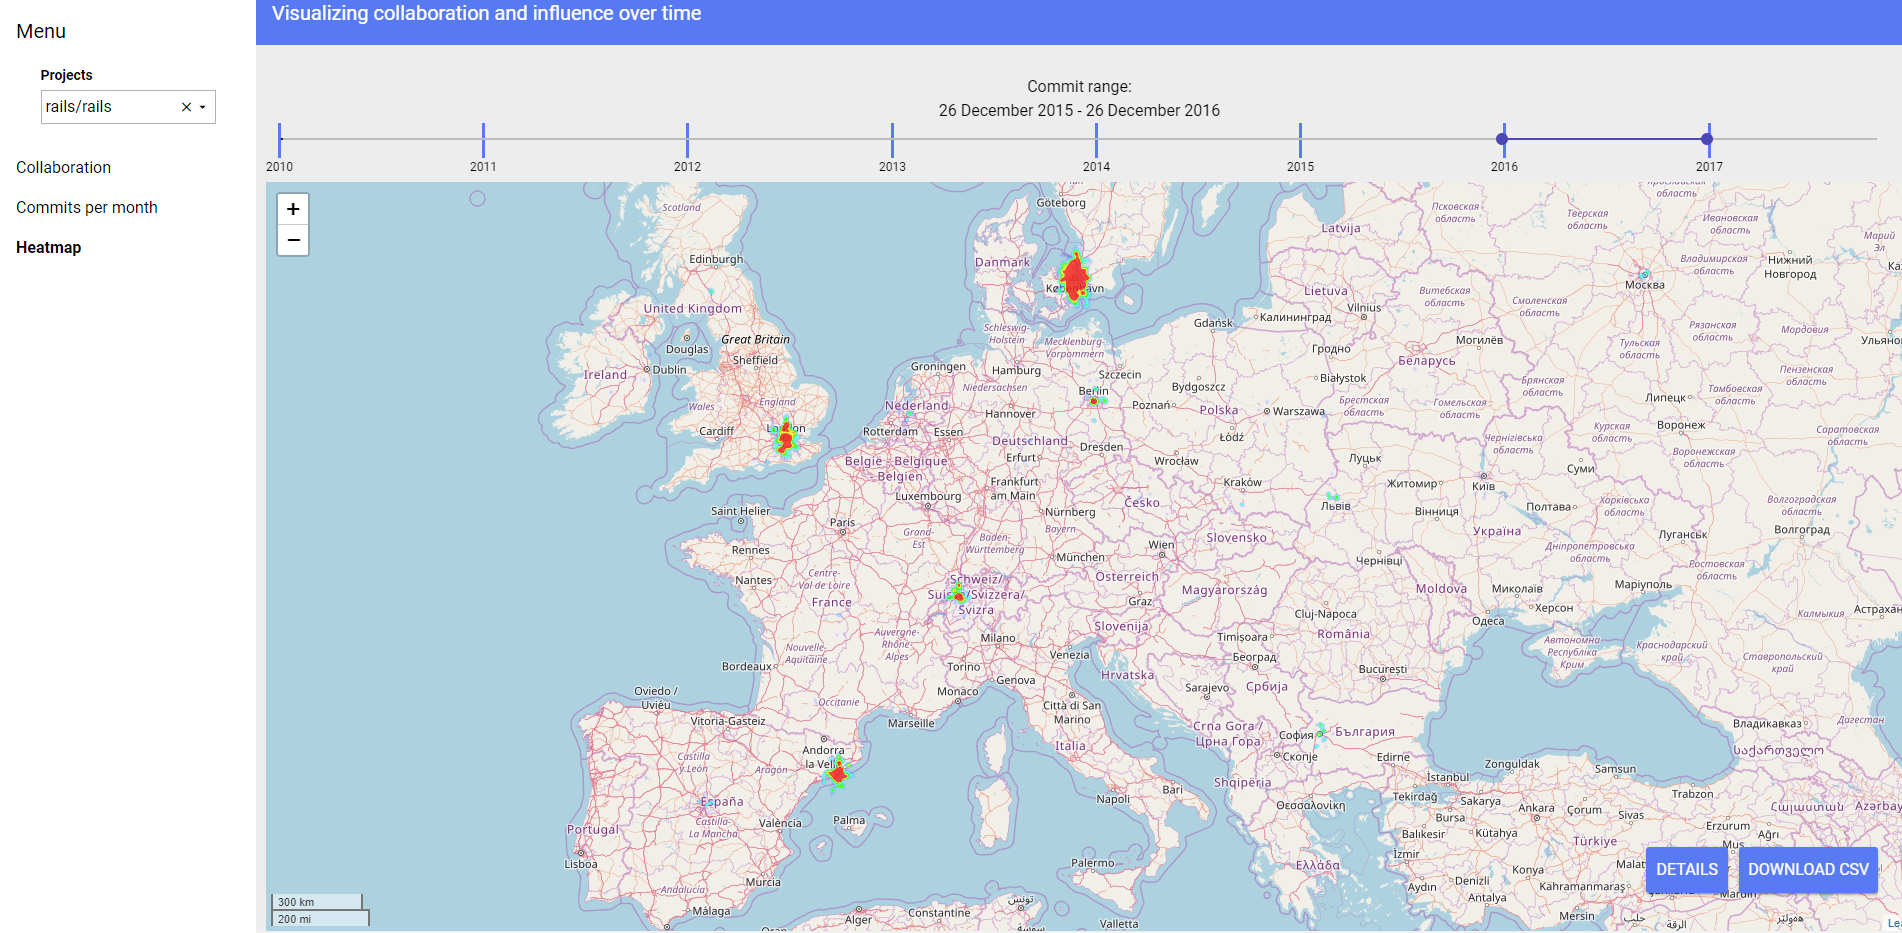
\includegraphics[scale=0.35]{images/rails-heatmap-2016-2017.PNG}}
\caption{Example visualization of heatmap for rails from 2016 till 2017 in Europe}
\label{fig:commits-heatmap}
\end{figure*}

The third visualization in the application is a heatmap and is shown in figure ~\ref{fig:commits-heatmap}.
As well as the visualization for commits per month, this visualization is created with the D3 library.
The heatmap visualization uses the same slider as the collaboration visualization.
The visualization creates a heatmap for the commits belonging to the selected timespan.
The heatmap visualizes commits by color ranging from green to red.
Here red spots mean locations with a lot of commits, and green spots are locations with fewer commits.

\subsection{Evaluation}
There are some shortcomings to the platform and visualization which must be taken into account when concluding statements on the data visualized. 
First, the top 1000 repositories are not updated anymore, this is a snapshot of data from September 2017. 
Second, locations are not mandatory to be filled in on Github, and it can also be modified by users to a non-existing city. A user is also able to specify 'home' as its location for example.
This means not all the data can be visualized, in fact, 50\% of the data we used did not contain a location.
Finally, the platform delivers results dynamically per timespan, but the type of relation is preset and defined in the backend of the application. 
Future improvements could enhance the platform by giving more parameters to the query to create an even more dynamic visualization.

\FloatBarrier
\section{Results}
Gathered data contains 1000 repositories with over 5 million commits belonging to 160.000 users.
Not all of the user gave information on their whereabouts, but about 84.000 did.
This means that it was possible to retrieve locations for just over 50\% of the gathered users.

\begin{figure*}
\frame{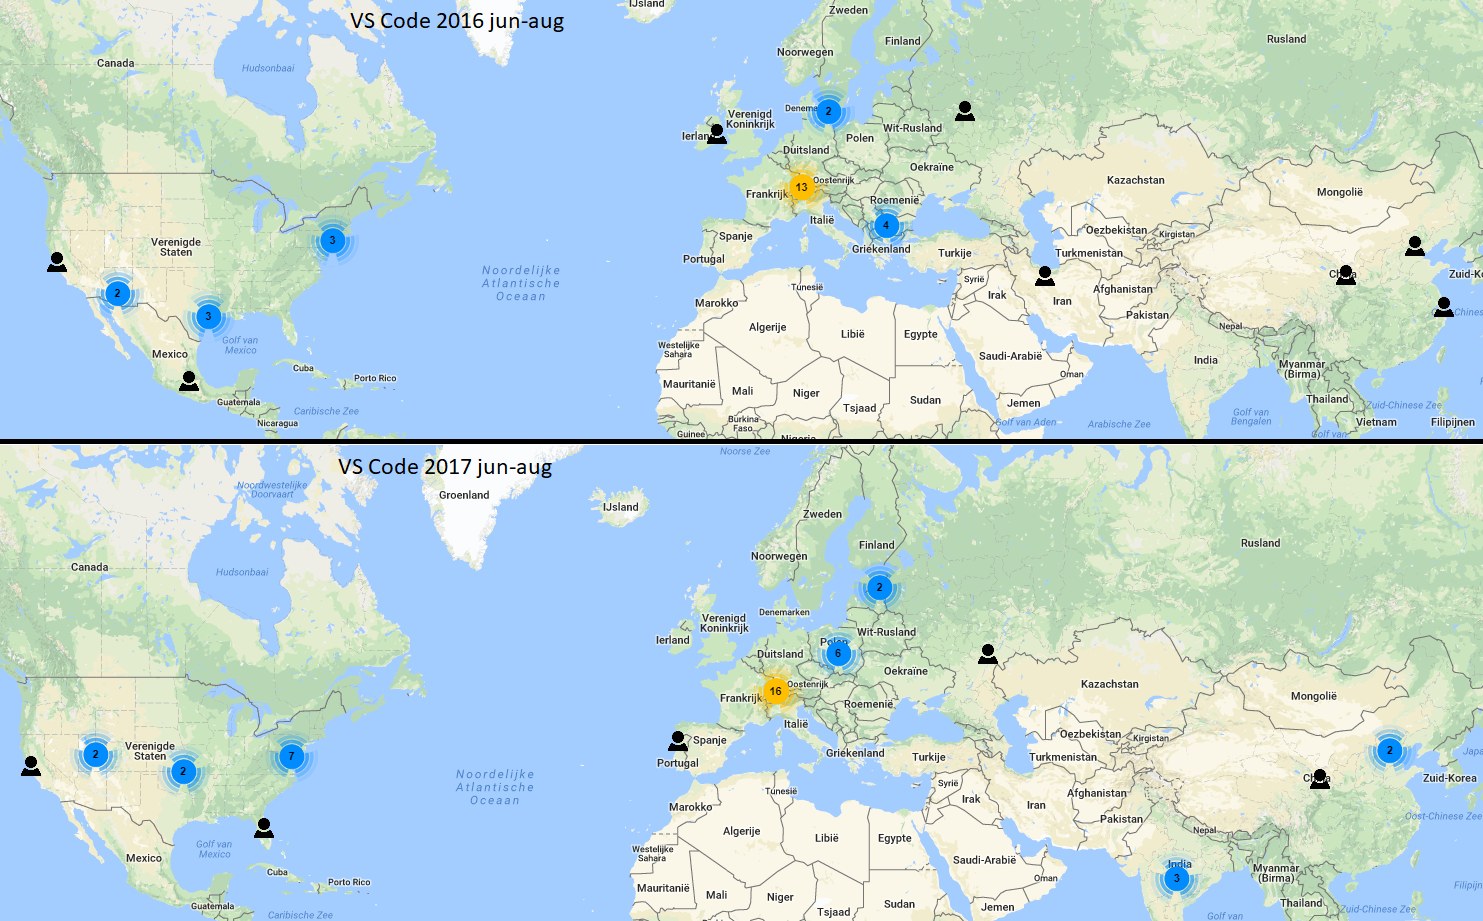
\includegraphics[scale=0.35]{images/results/developers-compared-vscode.PNG}}
\caption{Developer locations compared for VS Code in June-August 2016/2017}
\label{fig:vscode-developer-locations}
\end{figure*}

\begin{figure*}
\frame{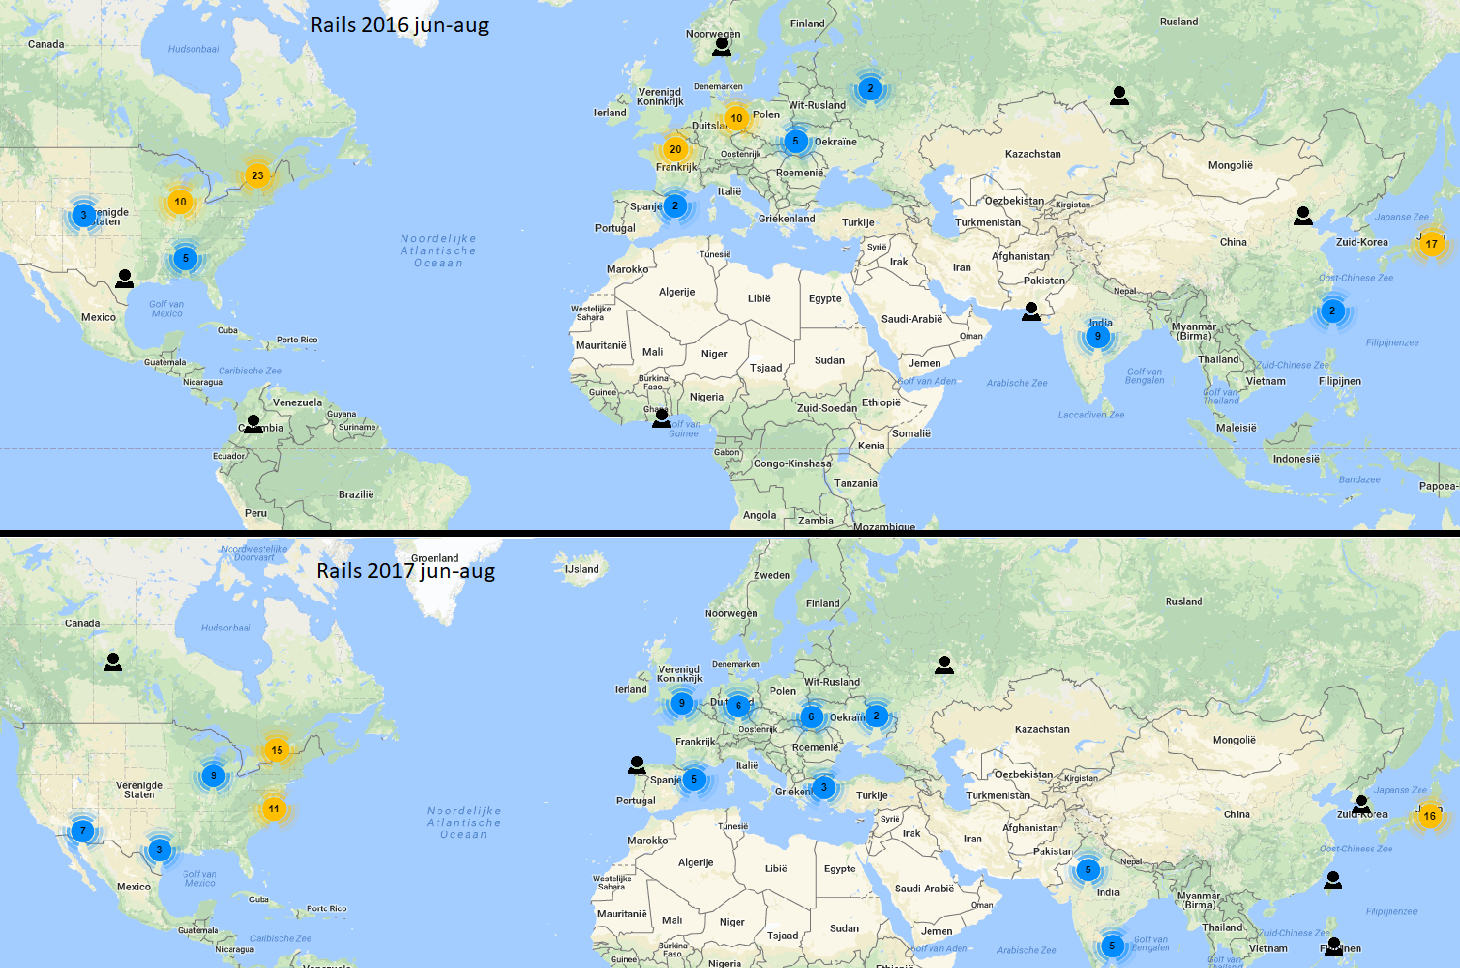
\includegraphics[scale=0.35]{images/results/rails-developers-compared.PNG}}
\caption{Developer locations compared for Rails in June-August 2016/2017}
\label{fig:rails-developer-locations}
\end{figure*}

By analyzing and visualizing multiple repositories using the platform some characteristics became visible for certain repositories.
Repositories backed by companies, such as React \cite{React}, Tensorflow  \cite{TensorFlow}, VSCode \cite{VSCode} have dedicated development teams.
Developers in such a team stay on the project for a relatively long time in contrast to popular repositories by normal users as shown in \ref{fig:vscode-developer-locations}.
Another characteristic for the company owned repositories is that there are less collaborators actually creating commits and originated from other regions than the dedicated development team.
Figure ~\ref{fig:vscode-developer-locations} and ~\ref{fig:rails-developer-locations} clearly show the difference between a company owned repository VS Code and Rails.
A Reason for the difference in amount of collaborators could emerge from the fact that there is already a core development team, making the threshold to join a project bigger.
Another reason could be the license companies use for open sourcing their software.

By using the heatmap and comparing time spans for different repositories, it is also clearly visible when popularity in a repository increases or decreases.
Looking at developer activity among several countries over time, there is not a noteworthy difference.
\textit{This means there are no countries visibly evolving faster in terms of developer activity.}

However, this shows that patterns can be found by visualizing repository data  and including a temporal component.

\begin{figure*}
\frame{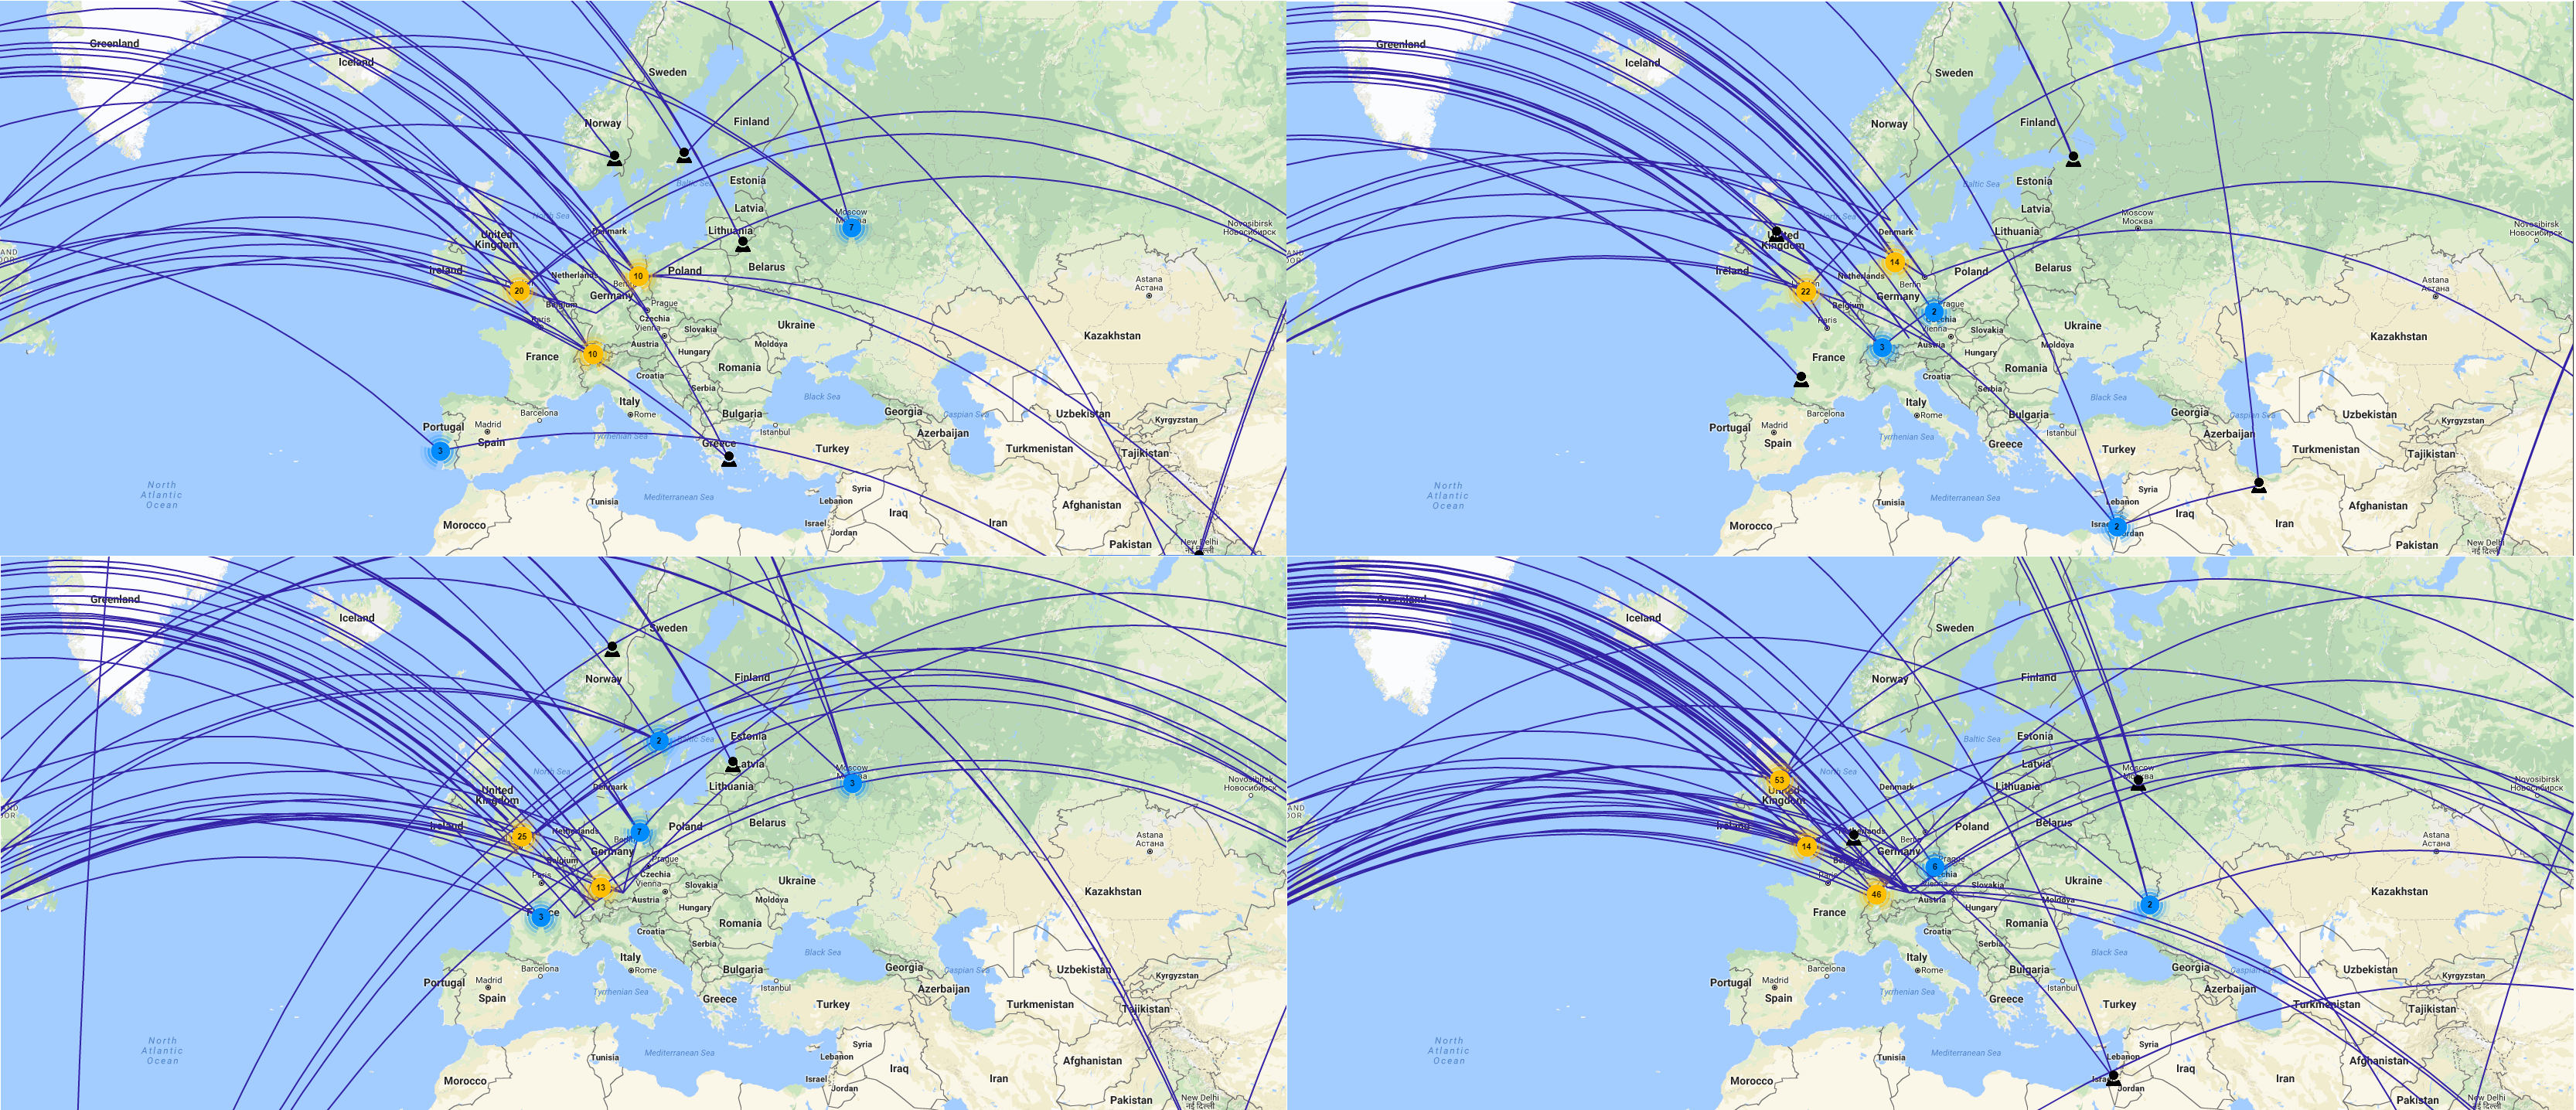
\includegraphics[scale=0.15]{images/results/tensorflow-2016Q1234-EU}}
\caption{Commits of TensorFlow per quarter in 2016 for Europe (Q1 top-left, Q2 top-right, Q3 bottom-left, Q4 bottom-right) }
\label{fig:tensorflow-2016}
\end{figure*}

Visualizing collaboration by including edges for consecutive commits between developers adds some interesting perspectives.
Users can instantly see where a lot of commits are created and are able to identify developers working together.
In addition, it is possible to identify where collaborating developers are working from, and which areas have strong collaboration links, depicted by a high number of edges.

After comparing collaboration links of repositories in the aforementioned dataset for different countries all over the world, \textit{there is no concluding evidence the number of commits made by developers evolve differently for different countries regardless of repository}.
However, when looking at individual repositories, a lot more can be said about evolution of commits per country.

In figure \ref{fig:tensorflow-2016} the commits made in Europe for TensorFlow \cite{TensorFlow} during 2016 are shown per quarter.
The top row depicts the first and second quarter, where the bottom row depicts the third and fourth quarter.
By examining these visualizations it is possible to find difference in the commits made by developers for different countries. 
Developers in The United Kingdom for example made 20 commits in the first quarter which slowly increases to 25 commits in the third quarter and ends at 67 commits by the end of the last quarter of 2016.
This means for 2016 the United Kingdom had an increasing amount of commits in 2016.
On the other hand Germany starts with 10 commits in the first quarter of 2016, which then increases to 14 commits in the second quarter, but decreases to zero commits in the last quarter of 2016.
This means that the overall commits made by developers from the United Kingdom increases in 2016, whereas the commits made by developers from Germany decreases in 2016.
This shows that the number of commits made by developers evolve differently for different countries in this particular example.
Now these developments in number of commits are identified, stakeholders can investigate underlying reasons.

\begin{figure*}
\frame{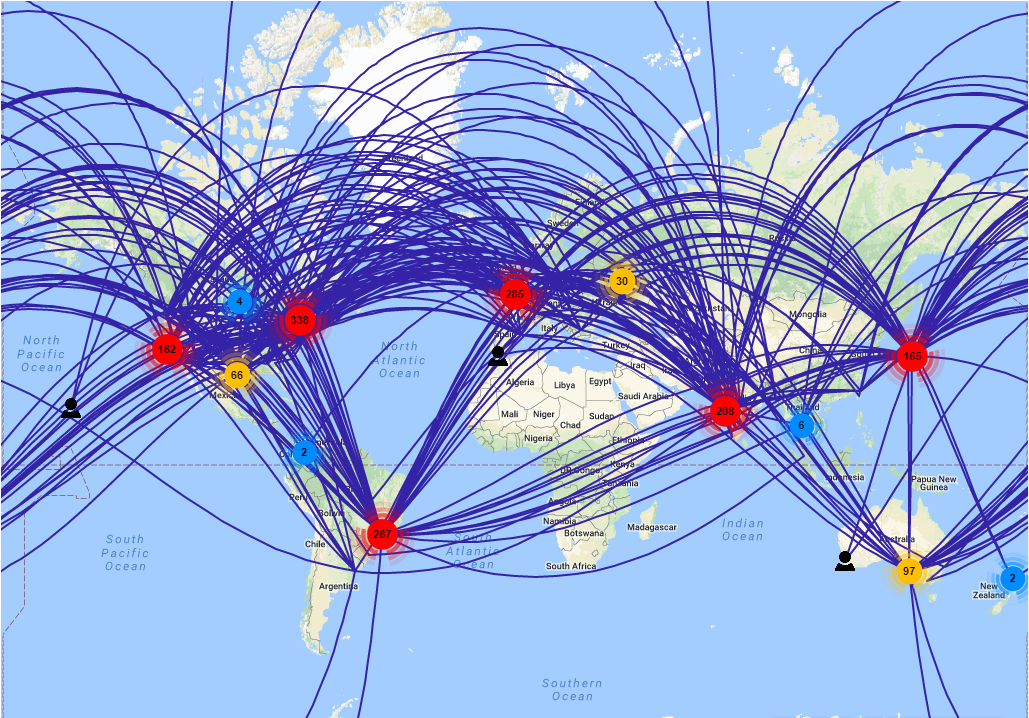
\includegraphics[scale=0.32]{images/results/rails-2016-Q1.png}}
\frame{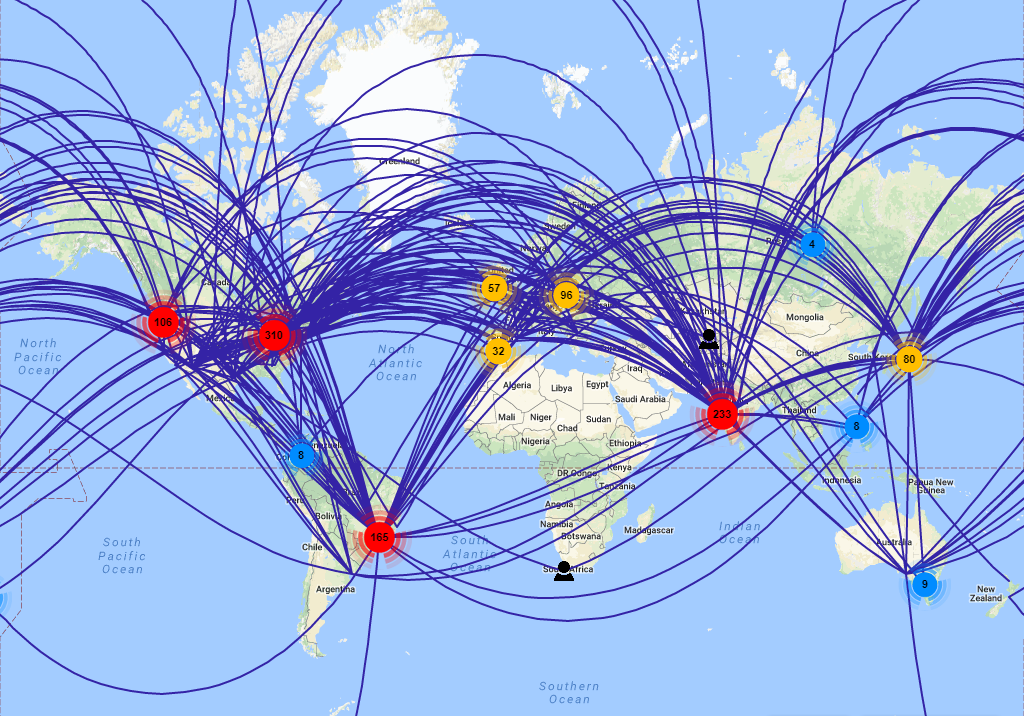
\includegraphics[scale=0.32]{images/results/rails-2016-Q2.png}}
\frame{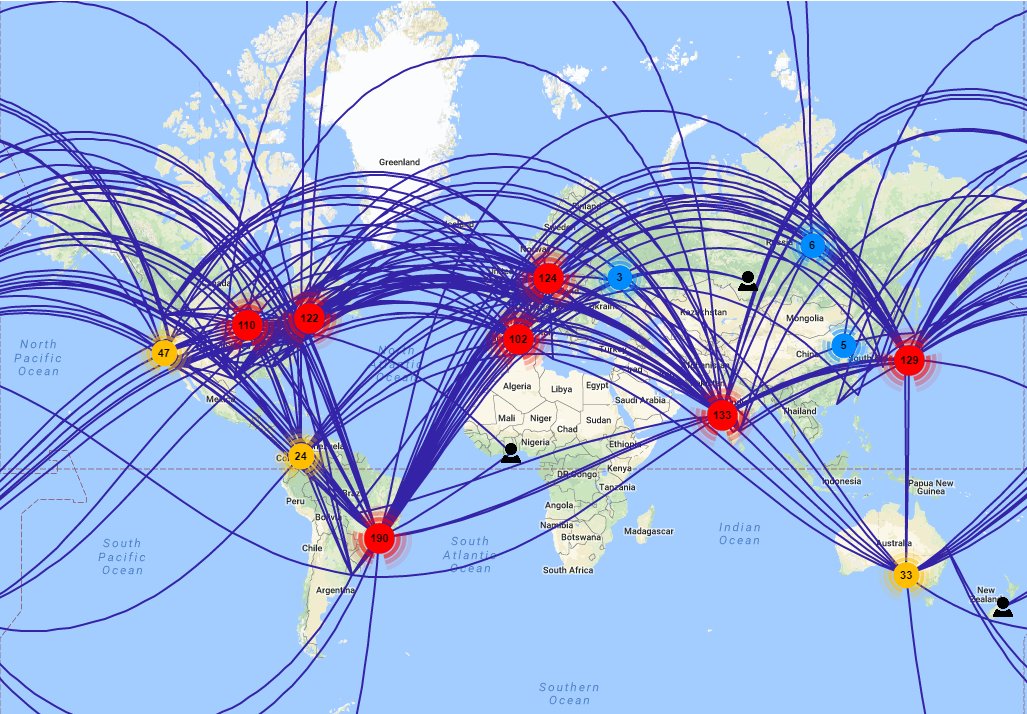
\includegraphics[scale=0.32]{images/results/rails-2016-Q3.png}}
\frame{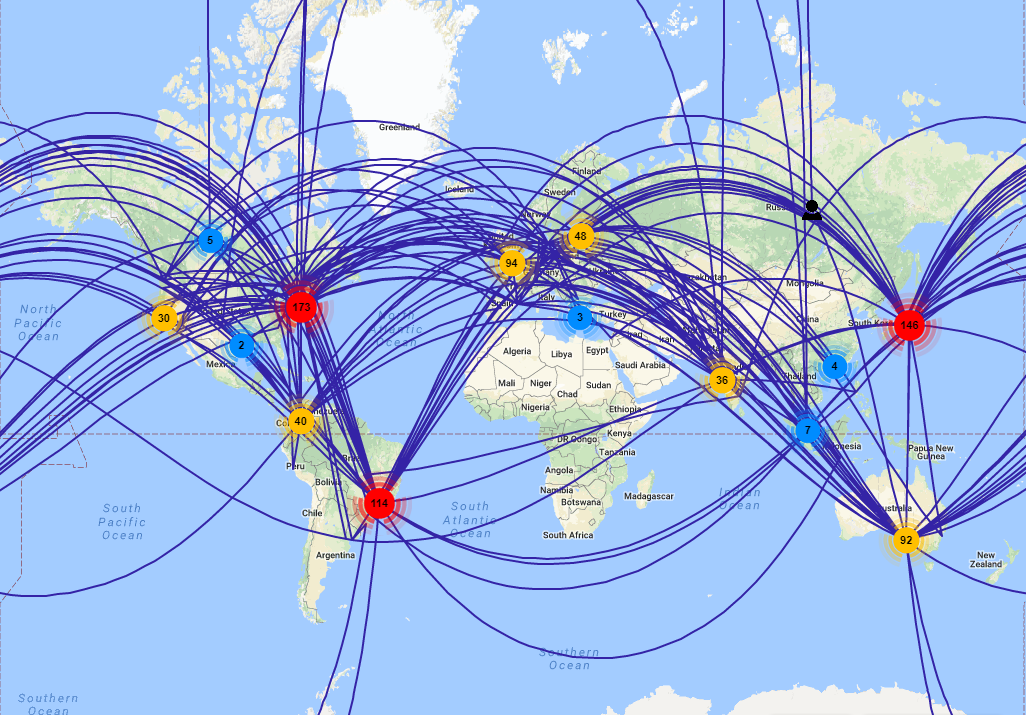
\includegraphics[scale=0.32]{images/results/rails-2016-Q4.png}}
\caption{Rails commits 2016 (Q1 top-left, Q2 top-right, Q3 bottom-left, Q4 bottom-right)}
\label{fig:rails-2016}
\end{figure*}

Another example on a broader scale, figure \ref{fig:rails-2016} depicts all the commits for the Rails \cite{Rails} repository over 2016 divided per quarter.
This repository has a large amount of contributors distributed all over the world.
Here, the largest number of commits for every continent was made in the first quarter, and there is a downward trend for all continents for the next three quarters.
This is probably due to the release of Rails 5.0, a major version change, on the 30th of June 2016, and has less to do with different countries having a different evolution pattern of number of commits made.

TensorFlow and Rails are two examples of the dataset on two different levels (country vs continent), but do illustrate there are definitely trends in number of commits made.
These trends however, are influenced more by individual repositories than they are influenced by countries.
So for a particular repository there could be a higher growth in number of commits per developer for a certain country/region, but for another repository the opposite is true.
This makes the evolution of number of commits fairly stable for a certain country/region, and invites to dig deeper into the data and start analyzing on a per repository basis.

\FloatBarrier
\cleardoublepage
\section{Discussion}
Visualizing repository data is an interesting way of looking at the data from a different perspective.
This leads to points of interest that otherwise wouldn't arise when looking at the raw data.
Introducing location data to the visualization adds a new dimension to analyze and form new hypotheses based this data.

\subsection{Limitations and threats to validity}
As stated, user location on GitHub is done on an opt-in basis, without any form of validation from the side of GitHub.
GitHub users are themselves responsible for entering valid locations in the field, and while it is possible to filter invalid locations it will always be a risk when used for research purposes.

\subsection{Future work}
In the future, more types of visualizations can be added, as well as more interaction through the use of the D3 library.
It is also interesting to include more detailed information about collaborating developers and the number of commits made.
In addition it would be of high value for stakeholders of a repository not listed in the used dataset to be able to import their repository in the web application itself, without having to resort to setup the project locally themselves.

\section{Acknowledgements}
We wish to thank the developer teams of all technologies used to build this application. 
The Go language and community made it possible to build a robust and fast data gatherer and accompanying API while Polymer enabled us to rapidly develop a web applications for everybody to use.
Also a big thank you to GitHub for providing open access to all data, and to D3 and Google for making it possible to build intuitive visualizations.

\bibliographystyle{ACM-Reference-Format}
\bibliography{bibliography}

\end{document}
